\section{Cellular Automata}
TODO rewrite to not repeat too much of the previous section

\textit{Cellular Automata} (CA) were first invented in the 1940s by von Neumann and Ulam as mathematical models of computation \cite{von-neumann-1966}.
They were inspired by biological organisms,
and created a model that could emulate some of their interesting and useful properties,
such as multi-cellular development (e.g. embryogenesis), reproduction (clonal or sexual) and robustness (e.g. self-repair).

In the following decades, as modern computers started to catch on,
the concept of CA became the basis for the field of \textit{Cellular Computing} (CC).
As the performance of "conventional" computers kept increasing dramatically,
CC never became the basis for the mainstream computers that we use today,
but CA and CC remained an area of research by mathematicians and computer scientists,
part of the larger field of \textit{artificial life}.
As the rate of this growth of performance diminished,
and parallel computing has shown itself to be difficult in practice,
some, such as Michael J. Flynn have speculated that CC might be the path forward \cite{flynn-1996} .
Matthew Cook proved that a CA of a certain configuration can be Turing complete \cite{cook-2004},
further fueling this idea.

A CA consists of a grid of very simple units called cells.
A cell can be in one out of a finite set of states.
Sipper \cite{sipper-1999} described the three core principles of CC, which also apply to CA in general:

\begin{description}
    \item[Simplicity]
        ~\\
        A cell is simple and can do very little by itself.
    \item[Vast Parallelism]
        ~\\
        The number of cells is very large, much more than the number of processors in a conventional parallel computer.
    \item[Locality]
        ~\\
        All interactions between cells take place on a purely local basis.
        No cell knows or controls the entire system.
\end{description}

The cells in a CA use the information that is available to them about their neighborhoods and some set of rules to transition from one state to the next.
Depending on the starting state of the whole system and the rules,
it is possible to observe interesting emergent or self-organizing behavior over time and space.
These interesting CA often find an \textit{attractor} \cite{gershenson-2004, wolfram1986theory}.
If a sequence of states repeat periodically it is called a \textit{cycle attractor}, and if the CA stabilizes into a permanent state is is called a \textit{point attractor}.

%There are many properties of CA and of cellular computing that can be varied to produce different results \cite{sipper-1999}.
%In this paper we will define some further properties of CA as:
%\begin{itemize}
%    \item Structured as a 1D or 2D cartesian grid of cells.
%    \item Having uniform cells, sharing the same transition rules.
%    \item Having a finite discrete set of states that cells can have.
%    \item Synchronously changing states for all cells.
%\end{itemize}

%Examples that fit into this narrower definition include Von Neumann's cellular automaton \cite{von-neumann-1966}, Wolfram's elementary cellular automata (TODO cite) and Conway's Game of Life (TODO cite Conway).

%Figure \ref{fig:110} illustrates "elementarty CA 110", which has this property.
%This is an 1D CA, with successive states transitioning from the top to the bottom over time.
%Two different patterns stand out from the background.
%Over time they move towards each other and interact.
%This interaction is used in Cook's proof that CA 110 is Turing complete.
%
%\begin{figure}
%\centering
%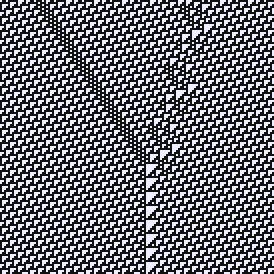
\includegraphics[width=\columnwidth]{img/110}
%\caption{Elementary CA 110
%(TODO cite \protect\url{https://commons.wikimedia.org/wiki/File:Ca110-interaction.png} properly)}
%\label{fig:110}
%\end{figure}

%Since the inception of CA by Ulam and Von Neumann in the 1940s \cite{von-neumann-1966},
%researchers have been interested in them for their biology-like properties and emergent behavior.
%Most implementations of CA have been formal mathematical works or simulations on conventional computers,
%but work has also been done with physical implementations using various substrates (TODO cite).
%
%In recent times the problem posed by the end of Moore's law and he difficulty of parallel computing with conventional architectures has caused cellular computing to become relevant again.
%Michael J. Flynn created Flynn's Taxonomy in 1966 \cite{flynn-1966}, describing different types of parallel systems.
%In 1996 he wrote a new article \cite{flynn-1996},
%outlining some of the difficulties that had hindered the expected parallel processing power that he and his peers had imagined back then.
%In this article he also described what he thought to be the road ahead, which is to represent problems in cellular form.

\subsection{Transition Rules}
\label{sec:transitions}
Langton \cite{langton-1990} formally defined finite CA as consisting of a finite set of cell states $\Sigma$ of size $K = |\Sigma|$,
a finite input alphabet $\alpha$, and a transition function $\Delta$.
Each cell has a $N$-sized neighborhood.
The number of possible neighborhoods can be expressed by equation \eqref{eq:kn}.

\begin{equation}\label{eq:kn}
    |\alpha| = |\Delta| = |\Sigma^N| = K^N
\end{equation}

The transition function for a CA must thus encode a mapping of $|\alpha|$ different inputs to one of $K$ states.
The number of possible unique transition functions is thus $K^{(K^N)}$.

Traditionally $\Delta$ has been encoded as a complete mapping $\Delta: \Sigma^N \rightarrow \Sigma$, which can be implemented as a lookup table.
When working with non-trivial CA where both $K$ and $N$ can be relatively large numbers,
it becomes a problem both to store the mapping $\Delta$ in an efficient way,
and the space of possible $\Delta$ becomes too large to be explored by exhaustive enumeration.

In studies of CA transition rules, it has been found that most rules lead to uninteresting behavior,
either falling into an "order" which is either static or repeating periodically,
or into chaos, where all useful information is quickly lost in noise.
It is in the critical border region between these behaviors that interesting behaviors and computation can occur \cite{langton-1990}.
But in order to find these interesting $\Delta$, a smart search heuristic is needed.

\subsection{The $\lambda$ Parameter and the Edge of Chaos}
TODO

\subsection{Morphology Problems}
TODO

